% Code from http://tex.stackexchange.com/questions/178800/creating-sections-each-with-title-pages-in-beamers-slides
\begin{frame}
	\vfill
	\centering
	\begin{beamercolorbox}[sep=8pt,center,shadow=true,rounded=true]{title}
		\usebeamerfont{title}\insertsectionhead\par%
	\end{beamercolorbox}
	\vfill
\end{frame}

\begin{frame}
	\frametitle{Random variables}
	A variable quantity whose possible values depend, in random manner, on a set of random outcomes events\footnote{\href{https://en.wikipedia.org/wiki/Random_variable}{Wikipedia}}\vspace{1em}
	
	Random variables are defined over \emph{probability spaces}: $(\Omega, \mathcal{F}, \mathcal{P})$\vspace{1em}
	
	Consider the toss of a coin\footnote{Additional information can be found, among others, in \href{http://vfu.bg/en/e-Learning/Math--Bertsekas_Tsitsiklis_Introduction_to_probability.pdf}{D.P. Bertsekas and J.N. Tsitsiklis. "Introduction to Probability"}}
	\begin{itemize}
		\item $\Omega=\{H, T\}$ is the set of possible outcomes. In this case head or tail
		\item $\mathcal{F}=\{\{\}, \{H\}, \{T\}, \{H,T\}\}$ is the set of events we consider
		\item $\mathcal{P}$ probability function. It associates elements of $\mathcal{F}$ with a probability value. For example $$\mathcal{P}(\{\})=0,\quad\mathcal{P}(\{H\})=0.5, \quad\mathcal{P}(\{T\})=0.5, \quad \mathcal{P}(\{H, T\})=1$$
	\end{itemize}
\end{frame}

\begin{frame}
	\frametitle{Moments}
	For a continuous random variable $X$, taking real values, and having probability density function $f(x)$ we have
	\begin{itemize}
		\item Mean: $\mu=E[X]=\int_\mathbb{R} sf(s)ds$
		\item $n$ moment: $\int_\mathbb{R} s^nf(s)ds$ 
		\item $n^{th}$ central moment $E[(X-E[X])^n]=\int_\mathbb{R} (s-\mu)^nf(s)ds$
		\item Variance: second central moment $E[(X-E[X])^2]=\int_\mathbb{R} (s-\mu)^2f(s)ds$
	\end{itemize}
	
	\vspace{1em}
	Not all random variables have moments of fine value. For example heavy-tailed distributions\footnote{\href{https://en.wikipedia.org/wiki/Heavy-tailed_distribution}{\small{ Wikipedia. Heavy-tailed distribution}}} 
	$$f(x)=\left\{\begin{aligned}
					\frac{1}{x^2} && x \geq 1\\
					0&&\textrm{otherwise}
				   \end{aligned}
	\right.$$
\end{frame}

\begin{frame}
	\frametitle{Mean and most likely outcome (mode)}
	\emph{Mean} and \emph{mode} are different concept
	\begin{itemize}
		\item Mean: weighted sum of all of the possible outcomes of the random variable
		\begin{itemize}
			\item Could be outside the set of the possible outcomes
		\end{itemize}
		\item Mode: An outcome having highest probability value
	\end{itemize}
	
	\begin{columns}
		\column{0.5\textwidth}
		Consider a random variable $X$ taking values
		\begin{itemize}
			\item 0 with probability 0.2 
			\item 1 with probability 0.8
		\end{itemize}
		\vspace*{1em}
	
	    Mean value: $\mu=0.2\cdot 0 + 0.8 \cdot 1=0.8$\vspace{0.5em}
	    
		Most likely outcome: $\displaystyle \argmax_{x\in\{0,1\}} p(x) \;=1$
		
		\column{0.4\textwidth}
		\begin{block}{Probability mass function of $X$}
			\centering
			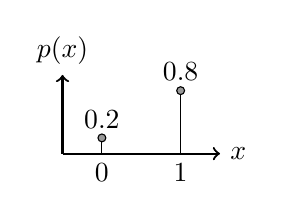
\begin{tikzpicture}
			%\draw[help lines, color=gray!30, dashed] (-4.9,-4.9) grid (4.9,4.9);
			\draw[->, thick] (-0.5,0)--(1.5,0) node[right]{$x$};
			\draw[->, thick] (-0.5,0)--(-0.5,1) node[above]{$p(x)$};
			\draw (0, 0) -- (0, 0.2) node [above] {$0.2$};
			\draw (1, 0) -- (1, 0.8) node [above] {$0.8$};
			\node [below] at (0,0) {0};
			\node [below] at (1,0) {1};
			\filldraw[fill=black!40, draw=black](0,0.2) circle (0.05cm);
			\filldraw[fill=black!40, draw=black](1,0.8) circle (0.05cm);
			\end{tikzpicture}
		\end{block}
	\end{columns}
	
	
	%Under certain assumptions (e.g., Ergodicity) the average of 
	
	\takeaway{The mean value is not even an element of the possible outcomes}
\end{frame}
\begin{frame}
	\frametitle{Sum of independent random variable}
	\onslide<1->The distribution of the sum of two random variables must always be carefully computed\vspace{0.5em}
	\begin{columns}\onslide<1->
		\column{0.5\textwidth}
		\begin{itemize}
			\item <1->$X$ uniform distributed between 0 and 1
			\item <1->$Y$ uniform distributed between 0 and 1
			\item <1->$Z=X+Y$ \emph{is not} uniform distributed between 0 and 1
			\item <2-> The distribution of $Z$ depends on the joint distribution of $X$ and $Y$
			\item <3-> If $X$ and $Y$ are independent variables, then $Z$ has a triangular distribution\\
			\begin{itemize}
				\item[] $X$ and $Y$ are independent if
				for all $x$  in $[0,1]$ and $y$ in [0,1] $$P(X=x,Y=y)=P(X=x)\cdot P(Y=y)$$	
			\end{itemize}	
		\end{itemize}
	
		\column{0.5\textwidth}
		\begin{block}{Probability distributions}
			\onslide<1->{
			\begin{tikzpicture}
				\draw[->] (-0.5,0)--(1.5,0) node[right]{$x$};
				\draw[->] (-0.5,0)--(-0.5,1.5) node[above]{$p(x)$};
				\draw[very thin, dashed] (-0.5, 1)node[left] {1} -- (0, 1);
				\draw[thin](0, 0) node[below] {0}-- (0, 1);
				\draw[thick] (0, 1) -- (1, 1); 
				\draw[thin] (1, 0)node[below] {1} -- (1, 1);
			\end{tikzpicture}}
			\onslide<3->{
			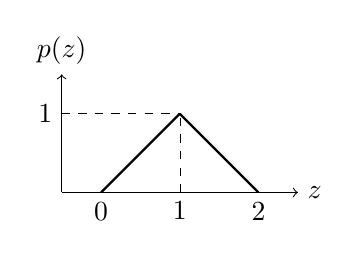
\begin{tikzpicture}
			\draw[->] (-0.5,0)--(2.5,0) node[right]{$z$};
			\draw[->] (-0.5,0)--(-0.5,1.5) node[above]{$p(z)$};
			\draw[very thin, dashed] (-0.5, 1)node[left] {1} -- (1, 1);
			\draw[thick](0, 0) node[below] {0}-- (1, 1);
			\draw[very thin, dashed] (1, 0)node[below]{1} -- (1, 1); 
			\draw[thick] (2, 0)node[below] {2} -- (1, 1);
			\end{tikzpicture}}
		\end{block}
	\end{columns}
\end{frame}
\begin{frame}
	\frametitle{The Gaussian distribution}
	The Gaussian distribution is also called \emph{normal} distribution and is denoted with the symbol $\mathcal{N}$\vspace{0.5em}
	
	The sum of independent normal random variables \emph{is normally distributed}
	\begin{itemize}
		\item $X$ and $Y$ are normally distributed; $X\sim\mathcal{N}(\mu_x, \sigma_x^2)$ and $Y\sim\mathcal{N}(\mu_y, \sigma_y^2)$
		\item $Z=X+Y$ is also normally distributed; $Z\sim\mathcal{N}(\mu_x+\mu_y, \sigma_x^2+\sigma_y^2)$
		\item <3-> If $\alpha$ is a non-zero constant, then $\alpha Z$ is normally distributed
		\begin{itemize}
			\item mean: $\alpha \mu_z$, variance: $\alpha^2\sigma_z^2$
		\end{itemize}
	
		\item <4-> If $\bm{Z}$ is a vector of jointly nominally distributed random variables with mean $\bm{\mu}_z$ and covariance $L=E[(Z-\bm{\mu}_z)(Z-\bm{\mu}_z)^T]$
		and $A$ is a matrix, then
		\begin{itemize}
			\item mean of $A\bm{Z}$ is $A \bm{\mu}_z$
			\item covariance matrix of $A\bm{Z}$ is $ALA^T$
		\end{itemize}
	\end{itemize} 
\onslide<4->{
\takeaway{\large Note that $X\cdot Y$ is \emph{not} normally distributed}}
\end{frame}
\begin{frame}
	\frametitle{Gaussian distributions and linear systems}
	Assume 
	\begin{columns}
		\column{0.6\textwidth}
		\begin{itemize}
			\item $X(0)$ is normal distributed $X(0)\sim\mathcal{N}(\mu_0, \sigma_0^2)$
			\item $W(k)$ is normal distributed $W(k)\sim\mathcal{N}(\mu_{w,k}, \sigma_{w,k}^2)$
			\item $X(0)$ and $W(k)$ are independent for all $k$
			\item for $k\geq0$ we have $X(k+1) =X(k) + W(k)$
		\end{itemize}	
		\column{0.4\textwidth}
		\begin{block}{Graphical representation}
			\begin{tikzpicture}
			\node(X0){$X(0)$};
			\node[above=1em of X0](W0){$W(0)$};
			\node[right=1em of X0](sum1){$+$};
			\node[right=1em of sum1](X1){$X(1)$};
			\node[above=1.2em of X1](W1){$W(1)$};
			\node[right=1em of X1](sum2){$+$};
			\node[right=1em of sum2](X3){$\cdots$};
			\draw[->] (W0) to (sum1);
			\draw[->] (X0) to (sum1);
			\draw[->] (sum1) to (X1);
			\draw[->] (W1) to (sum2);
			\draw[->] (X1) to (sum2);
			\draw[->] (sum2) to (X3);
			\end{tikzpicture}		
		\end{block}
	\end{columns}
	
	\vspace*{0.5em}

	\onslide<2-> What is the distribution of $X(1)$ ?
	\begin{itemize}\onslide<3->
		\item $X(1)$ is Gaussian distributed (sum of two gaussian variables)
		\item Mean $\mu_1=\mu_0+\mu_{w,0}$, variance $\sigma_1^2 = \sigma_0^2 + \sigma_{w,0}^2$
	\end{itemize}

	\vspace*{0.5em}
	\onslide<4-> What is the distribution of $X(k)$ ?
	\begin{itemize}\onslide<4->
		\item $X(k)$ is Gaussian distributed (sum of gaussian variables)
		\item Mean $\mu_k=\mu_0+\sum_{j=0}^{k-1}\mu_{w,j}$, variance $\sigma_k^2=\sigma_0^2 + \sum_{j=0}^{k-1}\sigma_{w,j}^2$
	\end{itemize}
\end{frame}

\begin{frame}
	\frametitle{Non Gaussian distributions and linear systems}
	Assume 
	\begin{columns}
		\column{0.6\textwidth}
		\begin{itemize}
			\item $X(0)$ is uniformly distributed $X(0)\sim\mathcal{U}(0, 1)$
			\item $W(k)$ is uniformly distributed $W(k)\sim\mathcal{U}(0, 1)$
			\item $X(0)$ and $W(k)$ are independent for all $k$
			\item for $k\geq0$ we have $X(k+1) =X(k) + W(k)$
		\end{itemize}	
		\column{0.4\textwidth}
		\begin{block}{Graphical representation}
			\begin{tikzpicture}
			\node(X0){$X(0)$};
			\node[above=1em of X0](W0){$W(0)$};
			\node[right=1em of X0](sum1){$+$};
			\node[right=1em of sum1](X1){$X(1)$};
			\node[above=1.2em of X1](W1){$W(1)$};
			\node[right=1em of X1](sum2){$+$};
			\node[right=1em of sum2](X3){$\cdots$};
			\draw[->] (W0) to (sum1);
			\draw[->] (X0) to (sum1);
			\draw[->] (sum1) to (X1);
			\draw[->] (W1) to (sum2);
			\draw[->] (X1) to (sum2);
			\draw[->] (sum2) to (X3);
			\end{tikzpicture}		
		\end{block}
	\end{columns}
	
	\vspace*{0.5em}
	
	\onslide<2-> What is the distribution of $X(1)$ ?
	\begin{itemize}\onslide<3->
		\item $X(1)$ has a triangular distribution
		\item Mean $\mu_1=\mu_0+\mu_{w,0}$, variance $\sigma_1^2 = \sigma_0^2 + \sigma_{w,0}^2\;$\footnote{\href{http://eli.thegreenplace.net/2009/01/07/variance-of-the-sum-of-independent-variables}{See also here}}
	\end{itemize}
	
	\vspace*{0.5em}
	\onslide<4-> What is the distribution of $X(k)$ ?
	\begin{itemize}\onslide<4->
		\item The distribution of $X(k)$ depends on the distribution of $X(k-1)$ and of $W(k-1)$
		\item Mean $\mu_k=\mu_0+\sum_{j=0}^{k-1}\mu_{w,j}$, variance $\sigma_k^2=\sigma_0^2 + \sum_{j=0}^{k-1}\sigma_{w,j}^2$
		
	\end{itemize}
\end{frame}

\begin{frame}
	\frametitle{Gaussian distributions and non linear systems}
	Assume 
	\begin{columns}
		\column{0.6\textwidth}
		\begin{itemize}
			\item $X(0)$ is normally distributed $X(0)\sim\mathcal{N}(0, 1)$
			\item $W(k)$ is normally distributed $W(k)\sim\mathcal{N}(0, 1)$
			\item $X(0)$ and $W(k)$ are independent for all $k$
			\item for $k\geq0$ we have $X(k+1) =X^2(k) + W(k)$
		\end{itemize}	
		\column{0.4\textwidth}
		\begin{block}{Graphical representation}
			\begin{tikzpicture}
			\node(X0){$X(0)$};
			\node[above=1em of X0](W0){$W(0)$};
			\node[right=1em of X0](sum1){$+$};
			\node[right=1em of sum1](X1){$X(1)$};
			\node[above=1.2em of X1](W1){$W(1)$};
			\node[right=1em of X1](sum2){$+$};
			\node[right=1em of sum2](X3){$\cdots$};
			\draw[->] (W0) to (sum1);
			\draw[->] (X0) to (sum1);
			\draw[->] (sum1) to (X1);
			\draw[->] (W1) to (sum2);
			\draw[->] (X1) to (sum2);
			\draw[->] (sum2) to (X3);
			\end{tikzpicture}		
		\end{block}
	\end{columns}
	
	\vspace*{0.5em}
	
	\onslide<2-> What is the distribution of $X(1)$ ?
	\begin{itemize}\onslide<3->
		\item $X(1)$ is not Gaussian distributed.
		\item Mean $\mu_1=E[X(0)^2]+\mu_{w,0}$
		\item Variance $\sigma_1^2=var(X(0))+\sigma_{w,0}^2$
	\end{itemize}
\end{frame}

\begin{frame}
	\frametitle{Few remarks}
	\begin{itemize}
		\setlength\itemsep{1.5em}
		\item Mean of the sum is always equal to the mean of the sum (linear operator)
		\item Variance of the sum is equal to the variance of the sum due to the assumption of independence
		\item Variables $X(k)$ are normally distributed for all $k\geq0$ \emph{only} in the case of linear systems and if the variables $w(k)$ are normally distributed
		\item If $X(k)$ is not normally distributed, knowing its mean and variance may not be sufficient for completely characterizing its distribution
	\end{itemize}  
\end{frame}

\begin{frame}
	\frametitle{Conditional distribution}
	Assume $X$, $Y$ are two random variables taking values in the interval $[0,1]$.\\ 
	For all $x,y$ the value of $P(X=x,Y=y)$ is known. The following probabilities can be computed
 	\begin{itemize}
 		\item <2-> Probability of $X$ taking value $x$ independently of the value taken by $Y$ $P(X=x)=\int_0^1 P(X=x, Y=z) dz$ (Marginal distribution)
 		\item <2->Probability of $Y$ taking value $y$ independently of the value taken by $X$ $P(Y=y)=\int_0^1 P(X=z, Y=y) dz$ (Marginal distribution)
 		\item <3->Probability of $Y$ taking value $y$ once we know that $X$ has value $x$ $P(Y=y|X=x)=\frac{P(X=x, Y=y)}{P(X=x)}$ (Conditional distribution)
 		\item <3->Probability of $X$ taking value $x$ once we know that $Y$ has value $y$ $P(X=x|Y=y)=\frac{P(X=x, Y=y)}{P(Y=y)}$ (Conditional distribution)
 	\end{itemize}
 	
\end{frame}

\begin{frame}
	\frametitle{Conditional distribution and expected conditional risk}
	Consider the case of estimating the value of a variable $X$ from its measurement $Y$
	Assume distribution of $X$ and of $(X,Y)$ is known
	\begin{columns}
		\column{0.6\textwidth}
		For example $Y=X+W$,\\ where $X\sim \mathcal{U}[3.0, 3.1]$ and $W\sim\mathcal{N}(0, 0.3)$\\\vspace{0.5em}
		The distribution of $X$ given the measurement $Y=3.05$ is the conditional distribution\\\vspace{0.5em}
		\onslide<2->
		How do we select a ``best'' \emph{value} from the distribution of $(X|Y=3.05)$?
		
		\onslide<1->
		\column{0.3\textwidth}
		\begin{block}{Random variables}
			\begin{tikzpicture}
				\node(X){$X$};
				\node[above=1em of X](W){$W$};
				\node[right=1em of X](sum){$+$};
				\node[right=1em of sum](Y){$Y$};
				\node[above =0.5em of W] (UnText) {Unknown};
				\node[right=1.5em of UnText] (MeasuredText) {Measured};
				\draw[->] (X) to (sum);
				\draw[->] (W) to (sum);
				\draw[->] (sum) to (Y);
				
				\begin{scope}[on background layer]
				\draw[fill=blue!10, rounded corners] ($(UnText.north west)+(-0.1,0.2)$)  rectangle ($(sum.south east)+(0.1,-0.2)$);
				\draw[fill=red!10, rounded corners] ($(Y.south west)+(-0.1,-0.2)$)  rectangle ($(MeasuredText.north east)+(0.1, 0.2)$);
				\end{scope}
			\end{tikzpicture}
		\end{block}
	\end{columns}
	\vspace{1em}
	
	The ``best'' value from $X|Y$ is the one that minimizes the expected conditional risk	$$R(z,y)=E[c(z-X)|Y=y]$$
\end{frame}

\begin{frame}
	\frametitle{Some properties of the conditional expectation}
	Assumptions:
	\begin{itemize}
		\item $c(z-x)$ is symmetric, e.g., $c(z-x)=(z-x)^2$
		\item the conditional distribution of $(X|Y=y)$ is symmetric around $E(X|Y=y)$
	\end{itemize}\vspace{1em}
	then
	\begin{itemize}
		\item the minimum of $R(z,y)$ does not depends on the specific cost function $c(z-X)$
		\item the minimum of $R(z,y)$ is given by $E[X|Y=y]$
	\end{itemize}\vspace{1.5 em}
		
	\takeaway{Under these assumptions mean and mode of the conditional distribution coincide}
\end{frame}